\documentclass{article}
<<<<<<< HEAD
\usepackage[UTF8]{ctex}
\usepackage{graphicx}
\usepackage[top=1cm, bottom=2cm, left=2.5cm, right=2.5cm]{geometry}
\usepackage[colorlinks=true, allcolors=blue]{hyperref}
\usepackage{float}


\title{实验报告1}
\author{伍紫涵}

\begin{document}
\maketitle

\begin{abstract}
本文是我学习的关于git的20个指示的实验报告,接下来我会详细地介绍我学习的内容,本文的LaTeX代码已经上传到了\href{https://github.com/qiqiqisi/Latex_Used.git}{github仓库}中,可以点击超链接进行查看。
\end{abstract}


{\hypersetup{hidelinks}\tableofcontents}


\section{git init}
git init的作用是建立一个仓库,在本地直观的体现就是所在文件夹中建立一个.git,把文件夹中的其他文件也包含在了仓库中。
\begin{figure}[H]
    \centering
    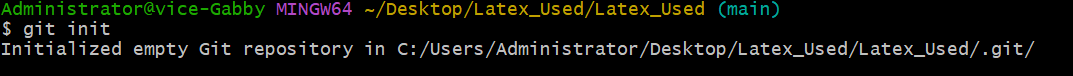
\includegraphics[width=1\linewidth]{git_init_code.png}
    \caption{git init运行图}
    \label{fig:init}
\end{figure}

\begin{figure}[H]
    \centering
    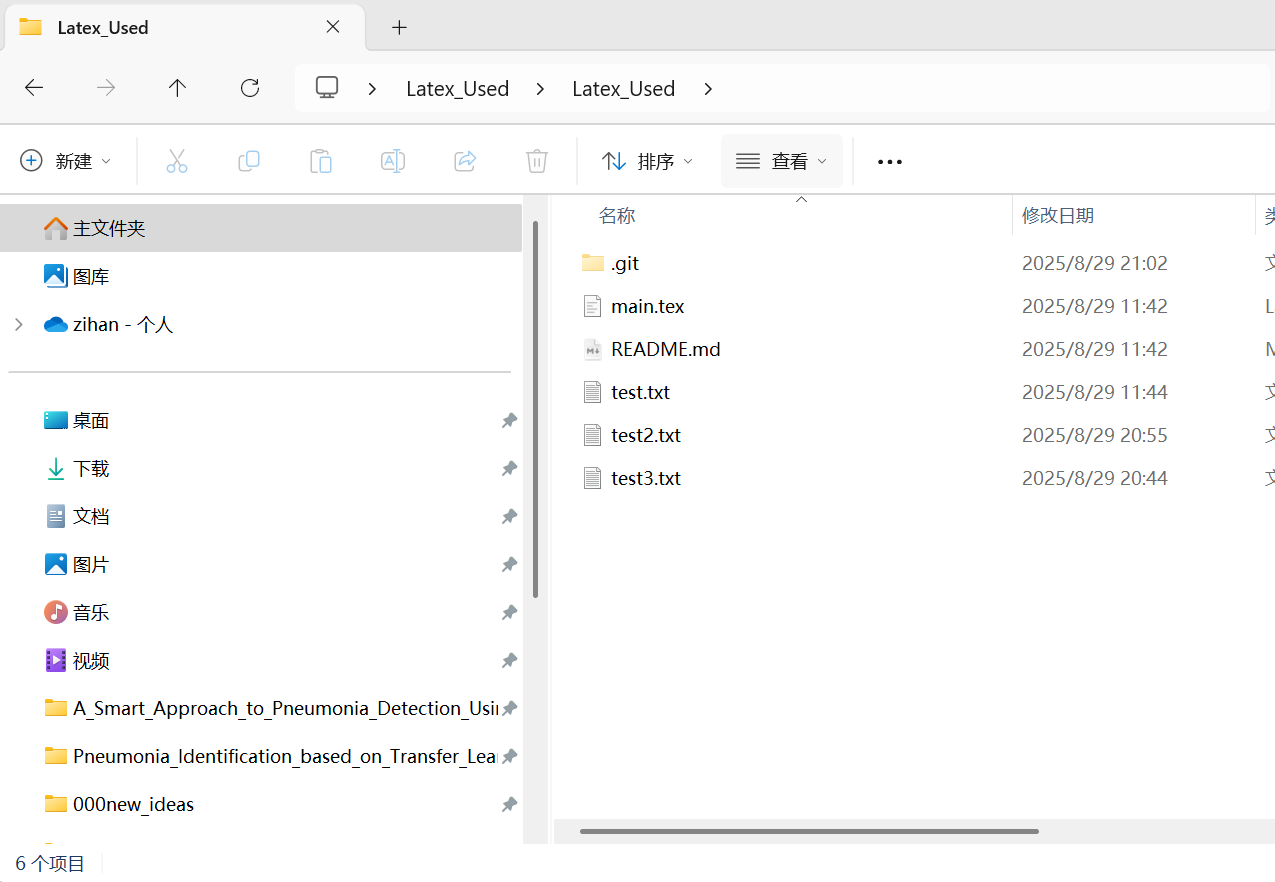
\includegraphics[width=1\linewidth]{git_init_show.png}
    \caption{文件夹中增加的.git}
    \label{fig:init1}
\end{figure}


\section{git help}
git help会列出所有git指示以及其作用。
\begin{figure}[H]
    \centering
    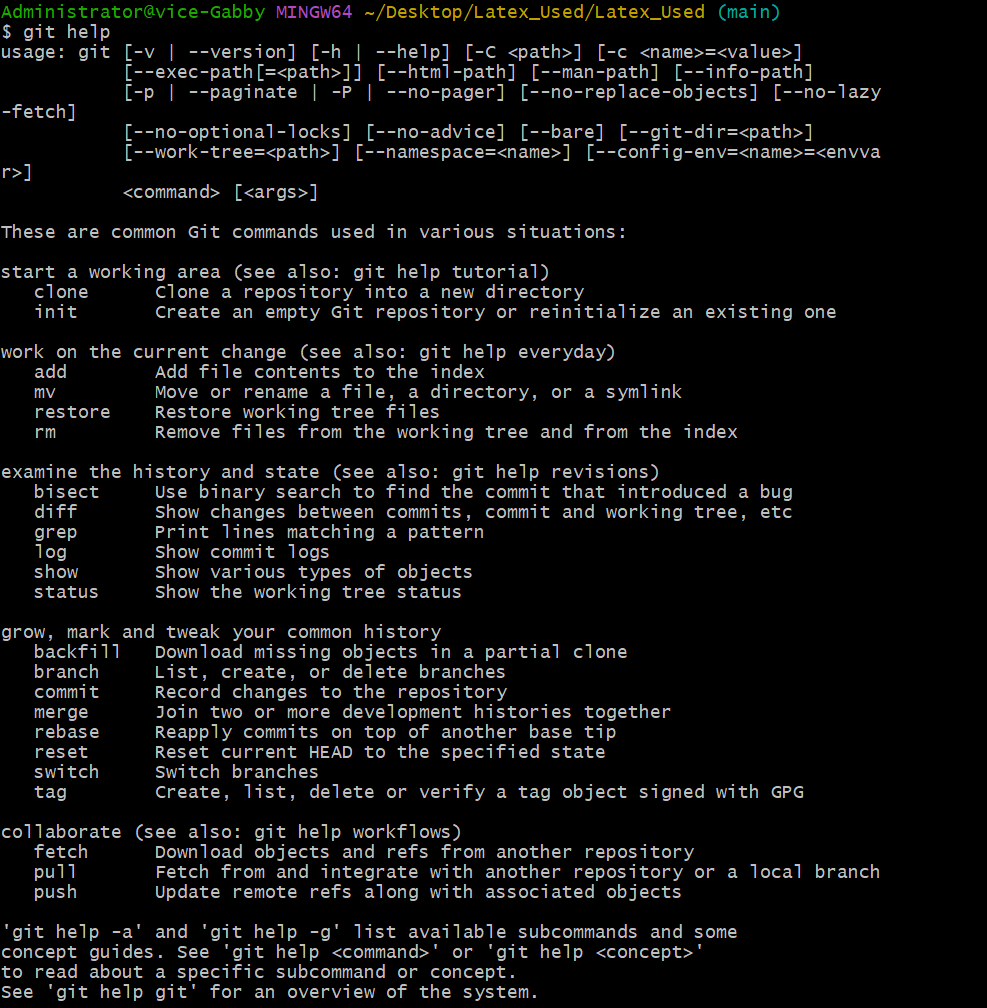
\includegraphics[width=1\linewidth]{git_help.png}
    \caption{git help运行图}
    \label{fig:help}
\end{figure}

\section{git clone <name>}
git clone <name>是把github上的仓库克隆到本地,首先需要找到github上的仓库链接然后再克隆。
\begin{figure}[H]
    \centering
    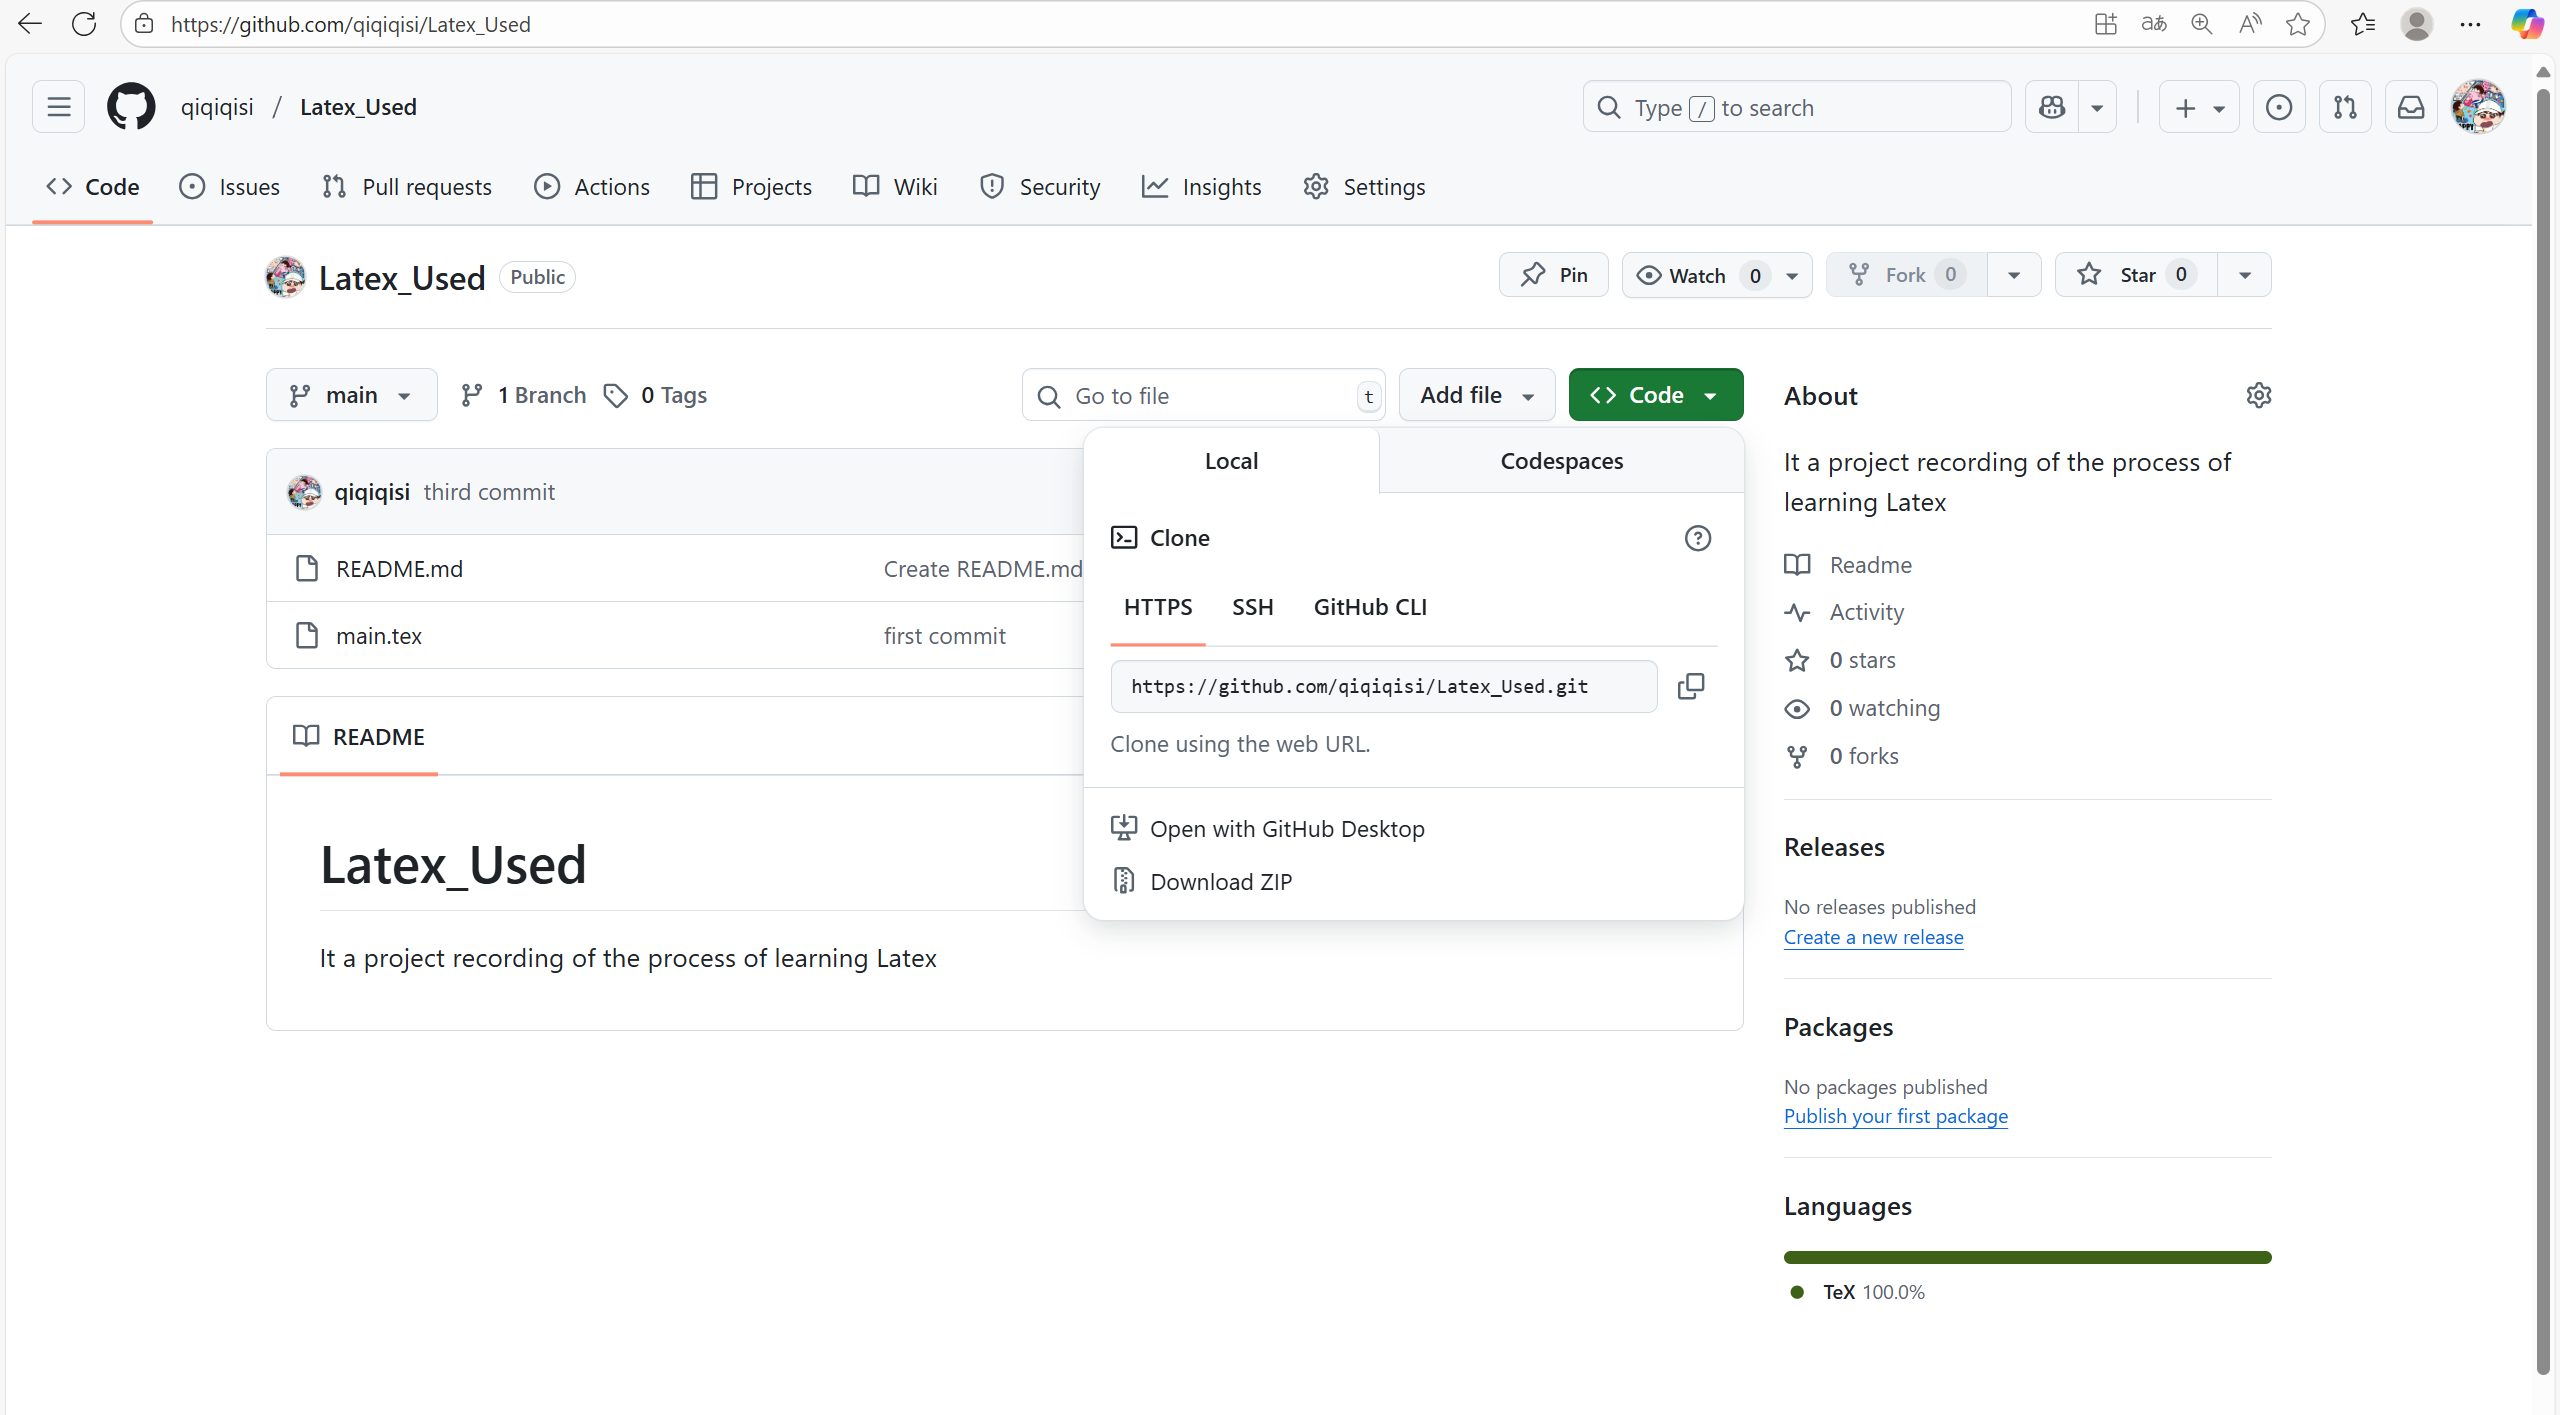
\includegraphics[width=1\linewidth]{find_github.png}
    \caption{github仓库界面}
    \label{fig:clone}
\end{figure}

\begin{figure}[H]
    \centering
    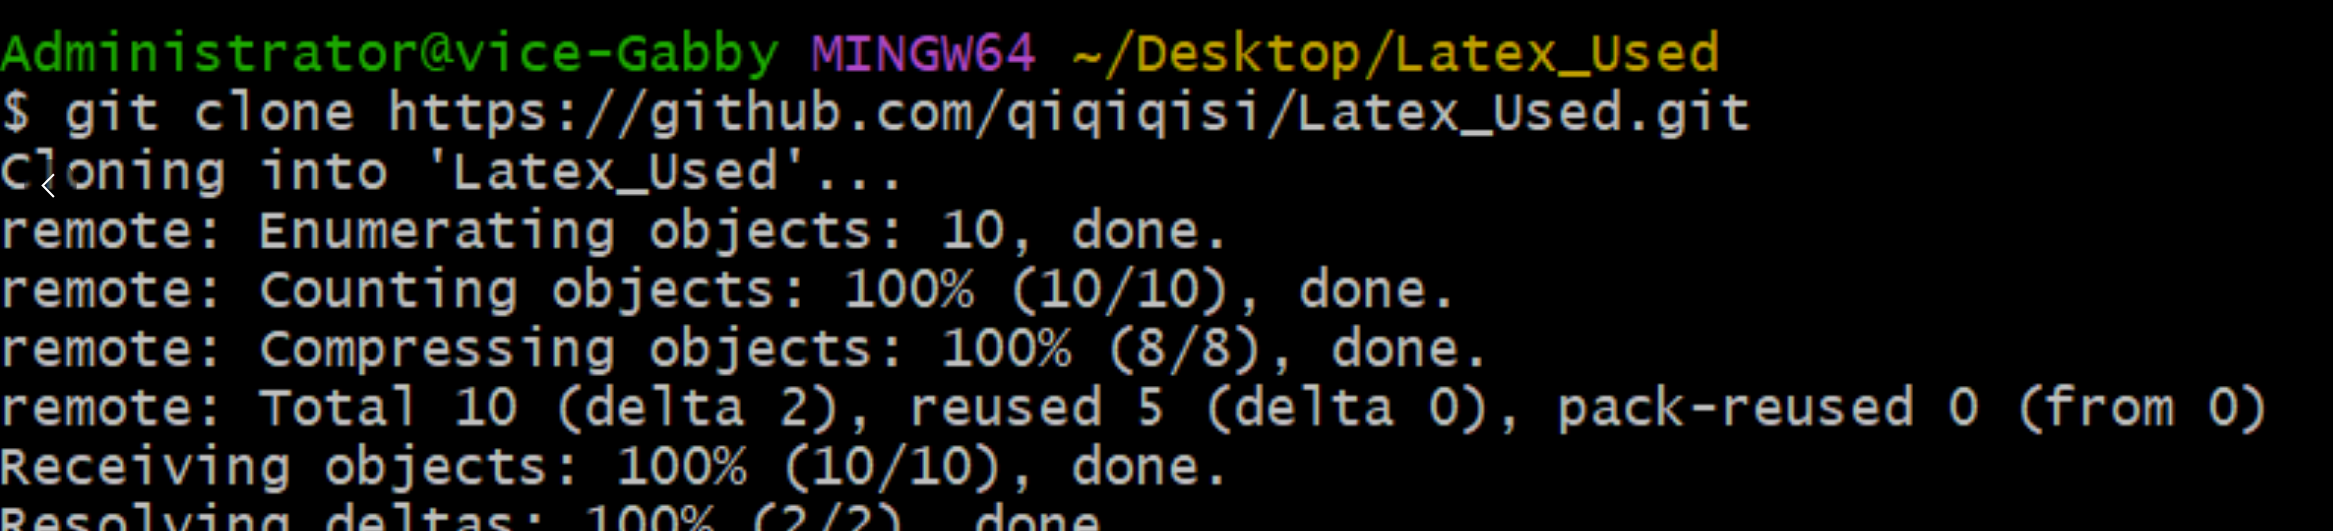
\includegraphics[width=1\linewidth]{git_clone.png}
    \caption{git clone <name>运行图}
    \label{fig:clone1}
\end{figure}

\section{git status}
git status可以查看仓库状态。
\begin{figure}[H]
    \centering
    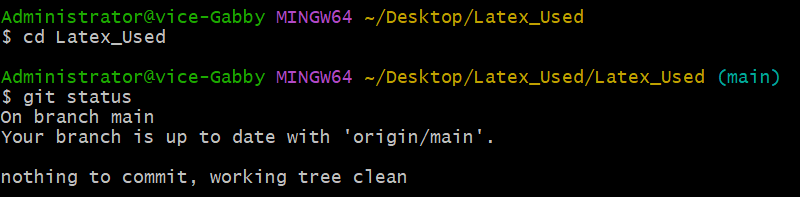
\includegraphics[width=1\linewidth]{git_status.png}
    \caption{git status运行图}
    \label{fig:status}
\end{figure}

\section{git add <name>}
git add <name>可以添加特定的文件到仓库中。
\begin{figure}[H]
    \centering
    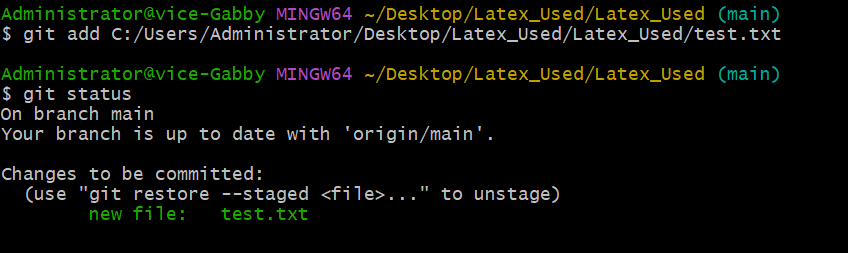
\includegraphics[width=1\linewidth]{git_add_name.png}
    \caption{git add <name>运行图}
    \label{fig:add}
\end{figure}

\section{git add .}
git add .可以把所有被添加在文件夹中的文件添加到仓库中去。
\begin{figure}[H]
    \centering
    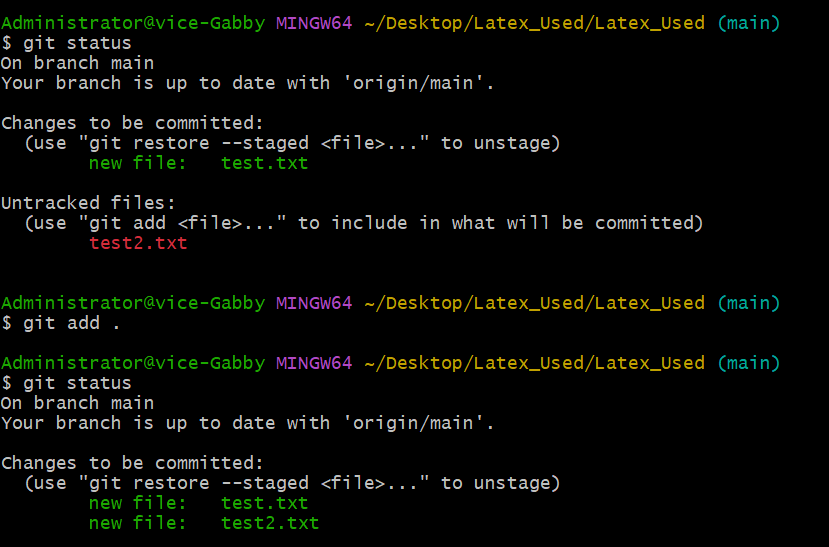
\includegraphics[width=1\linewidth]{git_add.png}
    \caption{git add .运行图}
    \label{fig:addall}
\end{figure}

\section{git commit -m <information>}
git commit -m <information>使用于说明简短的commit。
\begin{figure}[H]
    \centering
    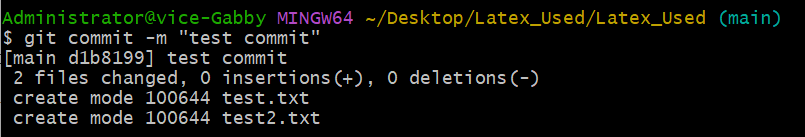
\includegraphics[width=1\linewidth]{git_commit.png}
    \caption{git commit -m <information>运行图}
    \label{fig:commit}
\end{figure}

\section{git push}
git push可以提交本地内容到github上的仓库上。
\begin{figure}[H]
    \centering
    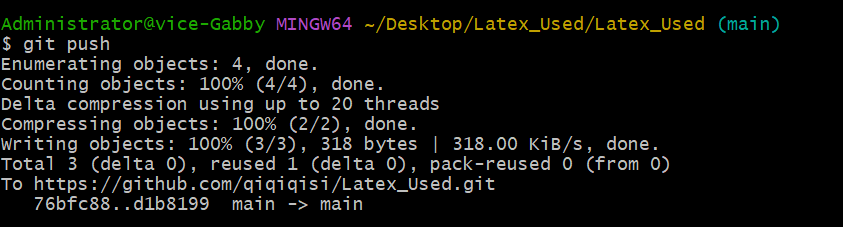
\includegraphics[width=1\linewidth]{git_push.png}
    \caption{git push运行图}
    \label{fig:push}
\end{figure}
\begin{figure}[H]
    \centering
    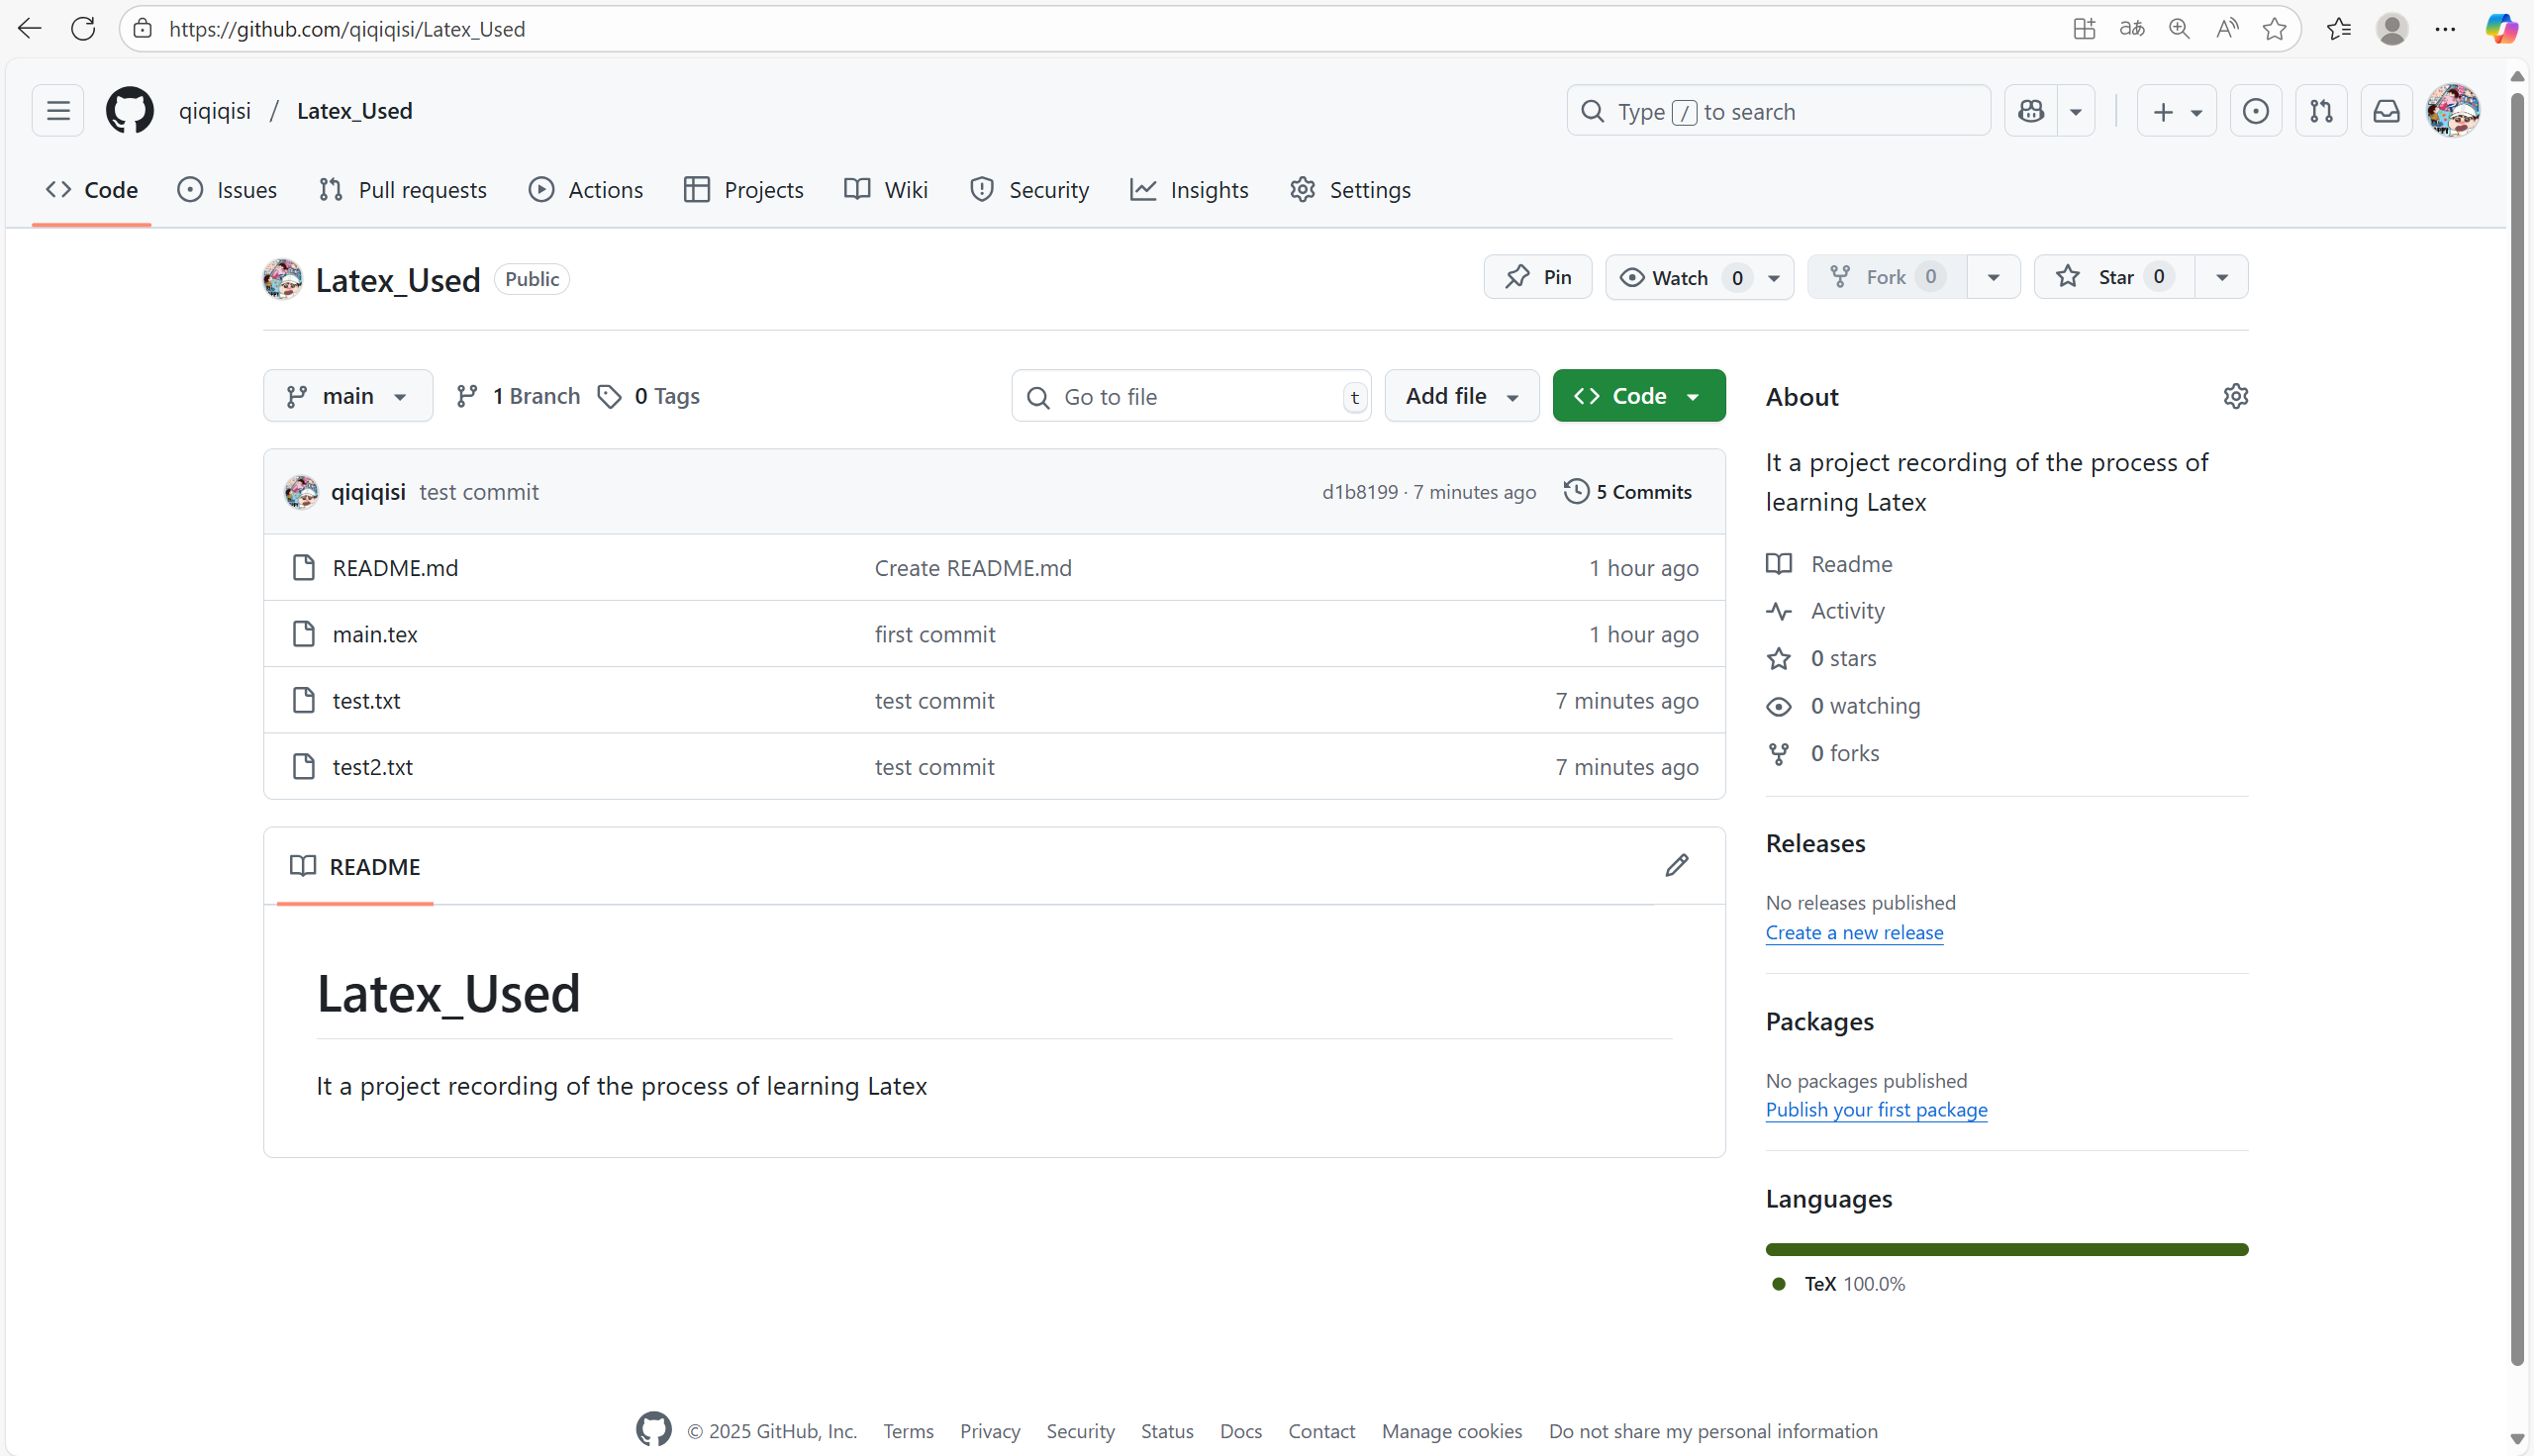
\includegraphics[width=1\linewidth]{push_result.png}
    \caption{git push运行后的github仓库展示}
    \label{fig:push1}
\end{figure}

\section{git log}
git log可以查看日志。
\begin{figure}[H]
    \centering
    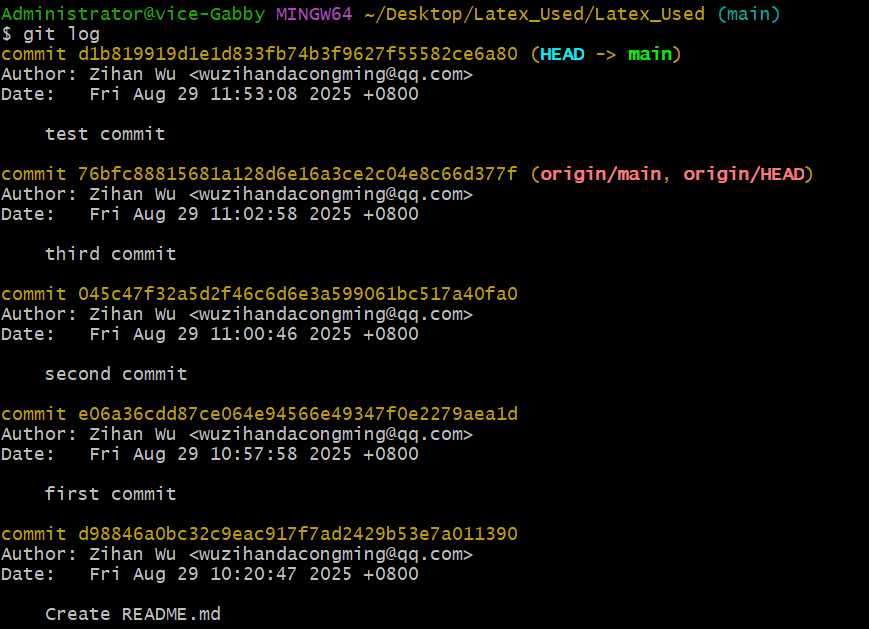
\includegraphics[width=1\linewidth]{git_log.png}
    \caption{git log运行图}
    \label{fig:log}
\end{figure}

\section{git log --all --graph --decorate}
git log --all --graph --decorate可以以图像化的方式显示所有历史提交。
\begin{figure}[H]
    \centering
    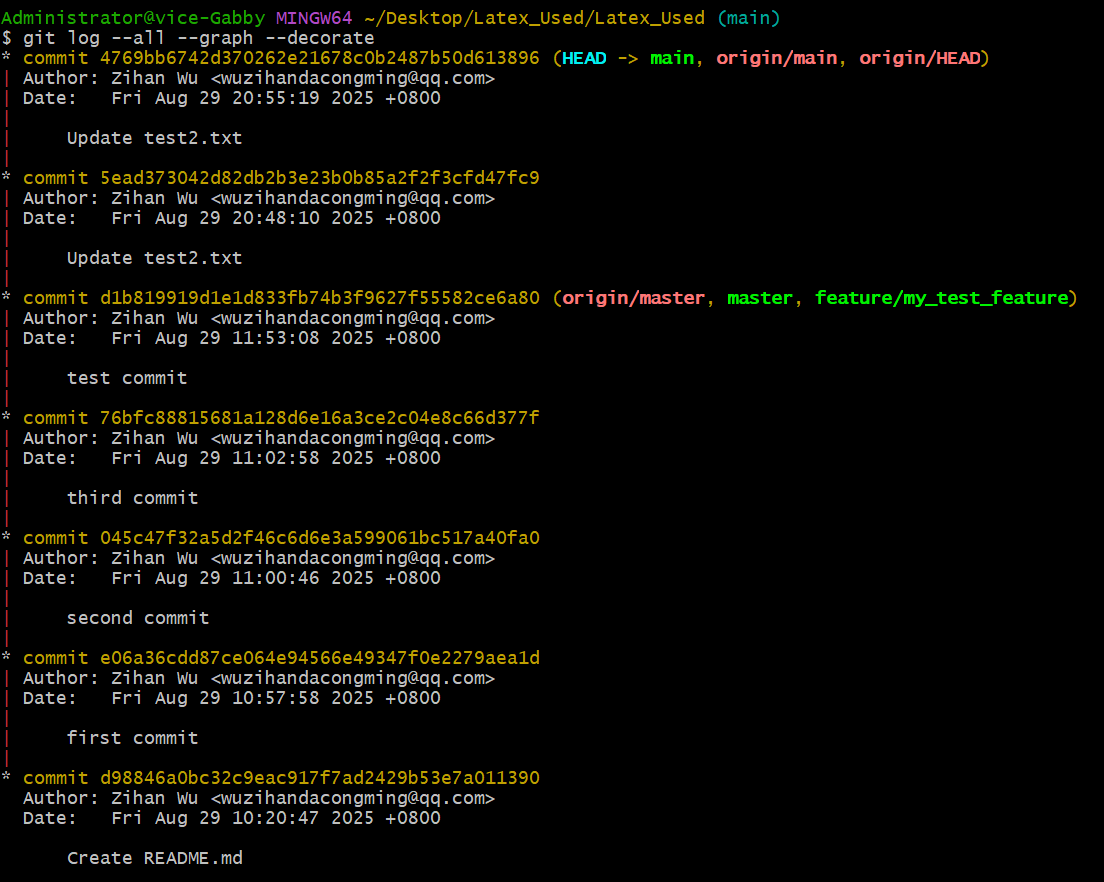
\includegraphics[width=1\linewidth]{git_log_decorate.png}
    \caption{git log --all --graph --decorate}
    \label{fig:log1}
\end{figure}

\section{git branch}
git branch可以查看分支。
\begin{figure}[H]
    \centering
    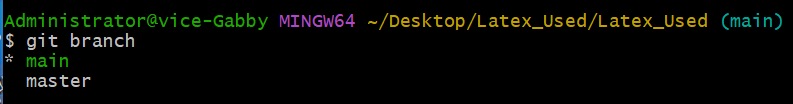
\includegraphics[width=1\linewidth]{git_branch.png}
    \caption{git branch运行图}
    \label{fig:branch}
\end{figure}

\section{git branch <name>}
git branch <name>可以创建分支。
\begin{figure}[H]
    \centering
    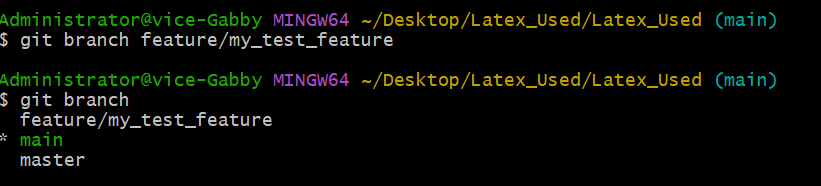
\includegraphics[width=1\linewidth]{git_branch_name.png}
    \caption{git branch <name>运行图}
    \label{fig:branch1}
\end{figure}

\section{git push -u origin <name>}
git push -u origin <name>将本地分支推送到github仓库中。
\begin{figure}[H]
    \centering
    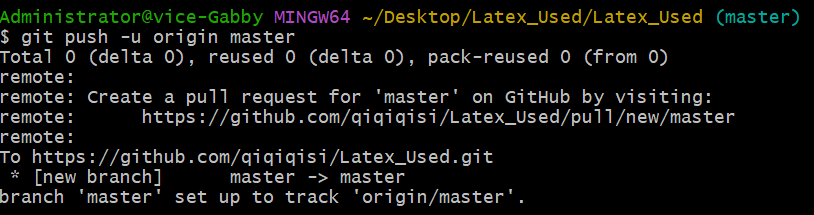
\includegraphics[width=1\linewidth]{git_push_branch.png}
    \caption{git push -u origin <name>运行图}
    \label{fig:pushfile}
\end{figure}

\section{git checkout <name>}
git checkout <name>可以转换分支。
\begin{figure}[H]
    \centering
    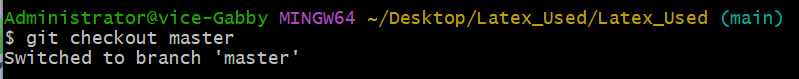
\includegraphics[width=1\linewidth]{git_checkout.png}
    \caption{git checkout <name>运行图}
    \label{fig:checkout}
\end{figure}

\section{git merge <name>}
git merge <name>可以和当前分支融合。
\begin{figure}[H]
    \centering
    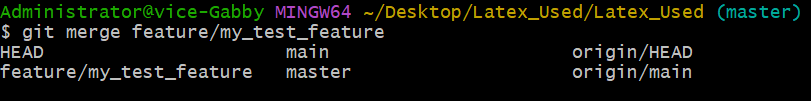
\includegraphics[width=1\linewidth]{git_merge.png}
    \caption{git merge <name>运行图}
    \label{fig:merge}
\end{figure}

\section{git remote}
git remote可以查看远程仓库名称。
\begin{figure}[H]
    \centering
    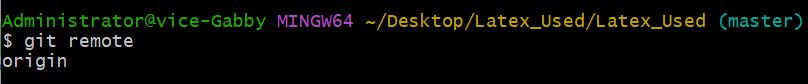
\includegraphics[width=1\linewidth]{git_remote.png}
    \caption{git remote运行图}
    \label{fig:remote}
\end{figure}

\section{git remote <name> <url>}
git remote <name> <url>可以添加新的远程仓库。
\begin{figure}[H]
    \centering
    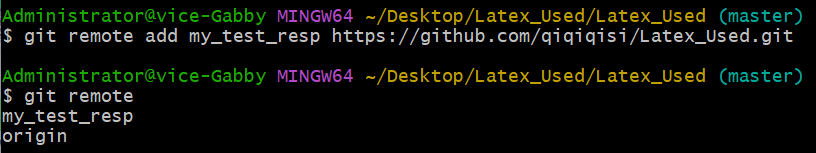
\includegraphics[width=1\linewidth]{git_remote_name.png}
    \caption{git remote <name> <url>运行图}
    \label{fig:remotename}
\end{figure}

\section{git pull}
git pull可以在github仓库上有新的修改的时候在本地的文件同步修改。
\begin{figure}[H]
    \centering
    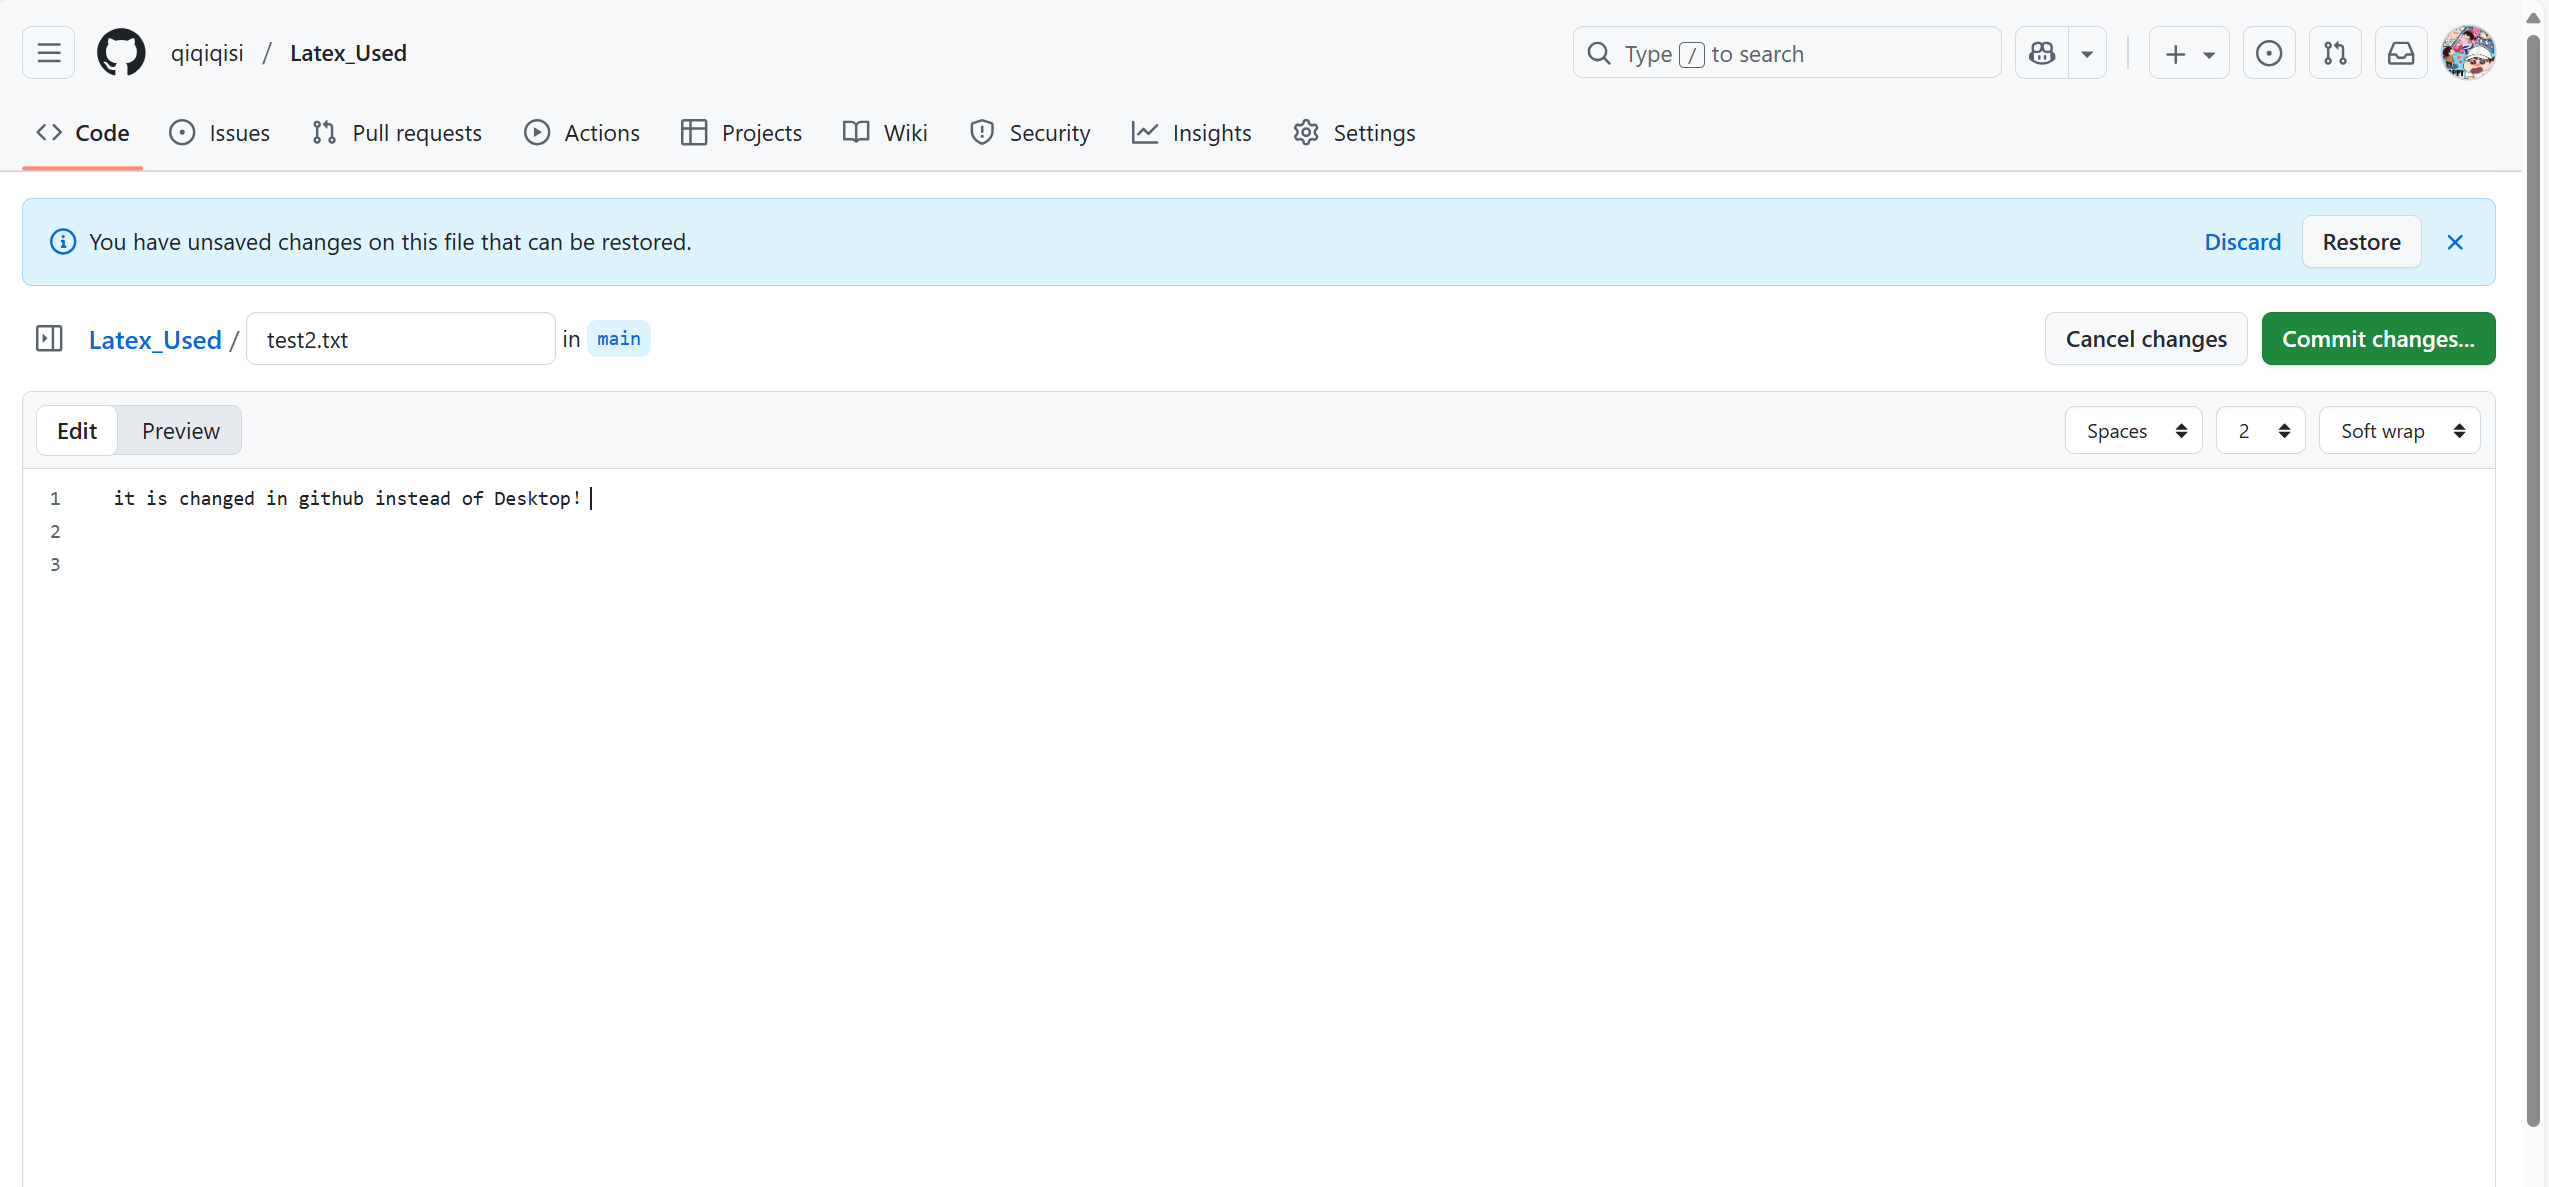
\includegraphics[width=1\linewidth]{github修改文件.png}
    \caption{在github上修改文件内容}
    \label{fig:pull}
\end{figure}
\begin{figure}[H]
    \centering
    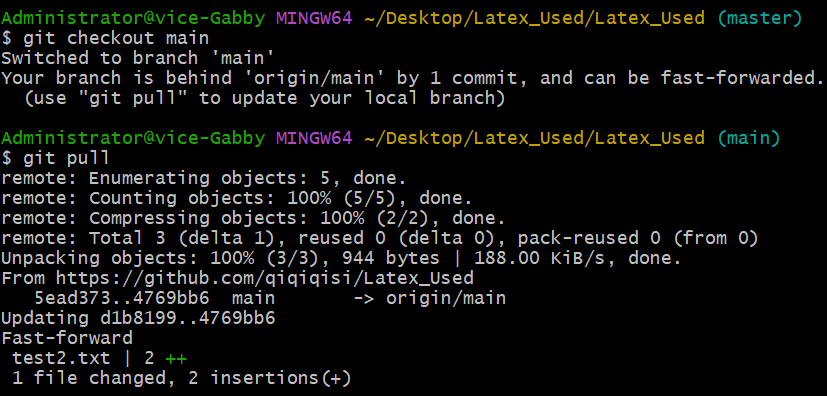
\includegraphics[width=1\linewidth]{git_pull.png}
    \caption{git pull运行图}
    \label{fig:pull1}
\end{figure}
\begin{figure}[H]
    \centering
    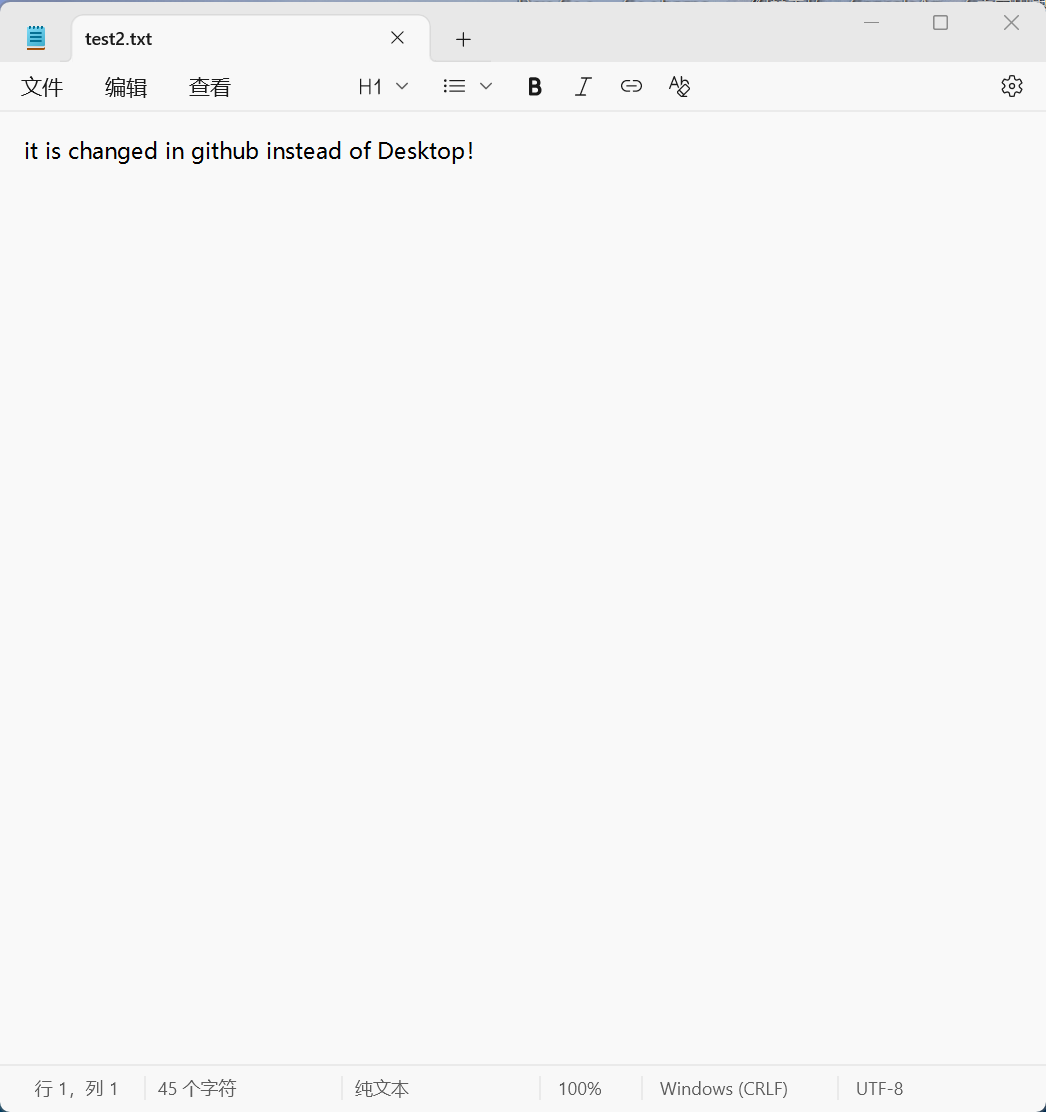
\includegraphics[width=1\linewidth]{本地文件.png}
    \caption{被更新的本地文件}
    \label{fig:pull2}
\end{figure}

\section{git blame}
git blame可以显示文件的修改信息。
\begin{figure}[H]
    \centering
    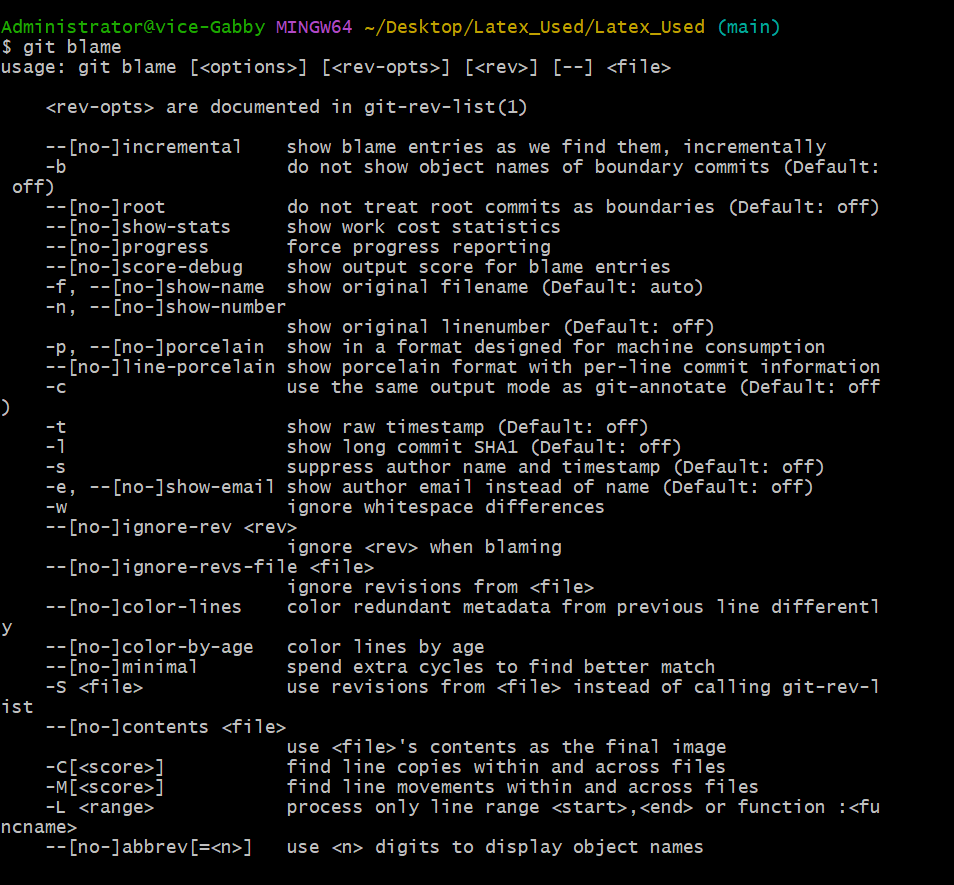
\includegraphics[width=1\linewidth]{git_blame.png}
    \caption{git blame运行图}
    \label{fig:blame}
\end{figure}

\section{git bisect}
git bisect可以用二分法快速查找引入bug的提交。
\begin{figure}[H]
    \centering
    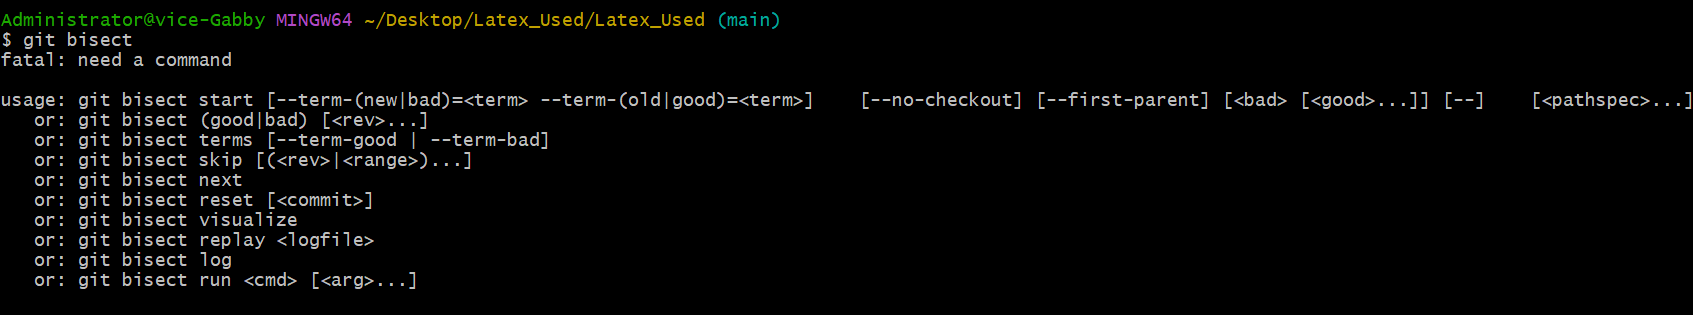
\includegraphics[width=1\linewidth]{git_bisect.png}
    \caption{git bisect运行图}
    \label{fig:bisect}
\end{figure}
=======
\usepackage{graphicx} % Required for inserting images

\title{example}
\author{zihan wu}
\date{August 2025}

\begin{document}

\maketitle

\section{Introduction}

>>>>>>> d1b819919d1e1d833fb74b3f9627f55582ce6a80
\end{document}
